\documentclass[12pt]{article}

\usepackage{notestyle}

\graphicspath{{./img/}}


\title{Notes Software Engineering}
\author{Brendon Mendicino}





\begin{document}

\maketitle
\newpage
\tableofcontents

\newpage
\section{TLS}
TLS (Transport Layer Security) is a message encrption protocol that is used to protect application level messages. TLS is the successor of SSL, which is now deprecated and should not be used, the TLS versions that are recomended are the lates TLS-1.2 and TLS-1.3. TLS as a protocol guarantees:
\begin{itemize}
  \item \textbf{Peer Authentication}: during a TLS session the server needs to compulsory authenticate himself, while for the client is not required, this is done using a challange-response which can \textbf{implicit} or \textbf{explicit}
  \item \textbf{Message Confidentiality}: each record can be \textbf{optionally} encrypted during the transmission
  \item \textbf{Message Authentication and Integrity}: every record sent in TLS \textbf{must} be authenticated and integrity needs to be guaranteed, this is done via a MAC
  \item \textbf{Replay and Filter Protection}: TLS uses an implicit sequence number which is included in the MAC
\end{itemize}
TLS is structured in two layers, the first one is \textbf{record protocol}, which manages the record exchange, the second one is composed on many ones:
\begin{itemize}
  \item \textbf{Handshake Protocol}: creates the TLS session
  \item \textbf{Change Cipher Spec}: change the encryption cipher suite 
  \item \textbf{Alert Protocol}: to signal the end a connection 
  \item \textbf{Application Data}: data coming from an application
\end{itemize}
In TLS all the keys for a connection are generated when a \textbf{session} is created with public key cryptography. The tow peers create a shared secred called \textbf{premaster secret} wiht PKC and by using some random numbers created by both the \textbf{master secreted} is created wich identifies a session, when a session is crated the peers can create multiple \textbf{connections} whose keys are generated using the master secret (key for MAC, key for encryption, IV for encryption), the reason why we have connection is done to reduce the overhead cause by the handshake. But using PKC to generated a session subject to attacks, in fact if someone stores all the messages and, in future, is able to find the private key is able the decrypt all the messages in the handshake, find the master secrect and decrypt all the exchanges messages, this is why \textbf{Perfect Foward Secrecy} was created, the key concept is: \textit{the compromise of a private key compromisises only the current and future traffic.}

In order to implement PFS we use an \textbf{ephemeral machanism}, we need auth of the server vie his certificate, the key of the server certificate must be marked as signature key, during the handshake the server will create another key-pair, to prove that the key comes from the server that is signed by the server, like if the server was a certificate authority, now the client has this new key the server can compute the premaster secret and send it encrypted to the client (with the new key-pair generated on the fly). Usaully the key-pair generated are done with DH, on the other hand RSA is not suitable because it is slow, so those keys may be reused due to performance issues, which can lead to attacks.

\subsection{TLS-1.2 Handshake}

\paragraph{Client hello:}
\begin{itemize}
  \item Contains the TLS version
  \item 28 randon bytes
  \item session id: == 0: new session, != 0: resume a previous session
  \item list of cipher suites (algos wiht enc + key exchenge + integrity), supported by the client
  \item list of compression methods supported by the client
\end{itemize}



\paragraph{Server hello:}
\begin{itemize}
  \item Version chosen by the server (should be strong), the server may choose to close the connection if the sercurity is too poor (old versions of TLS, old poor chipher suite), in TLS the security is chosen by the server, he decides wheter the algorithms are good enough
  \item 28 randon bytes
  \item session id: new session if the client id=0, or replace the old one if the server chooses to, this could be due to load balancing, in this scenario sharing the master secret could lead to overloading or vulnerabilities
  \item cipher suite chosen (should be strong): the server can refuse the connection if the cipher suite is too poor
  \item compression method chosen
\end{itemize}

\paragraph{Cipher suite:}
List of strings containing the various algorithms for: key exchange, symmetric encryption, hash, it is maintained by the IANA and the list arrives up to 200 items.

\paragraph{Certificate (server):}
If this is a new session the server is sending a X.509 certificate, with the whole chain of certifactes except for the root CA (that should be owned by the user), in the subject/subectAltName the certificate must contain the name of the server. This can be used for signing or for encryption, if the key is used for signature the \textit{Server Key Exchange} phase is required.

\paragraph{Certificate request (server): }
The server request to the client his certificate, along with a list of supported CAs.

\paragraph{Server key exchange:}
This message is only sent in case of explicit response to the challange, this can only happen when the server pubkey is eligible for signing, the next step is to use ephemeral DH (or ephemeral RSA) by signing the public parameters sent to the user (it is also possible to use anonymous DH whitout signing it, but it is subject to man in the middle attack), thus creating the premaster secret which are the parameters of the DH.

\paragraph{Certificate (client):}
Sends client certificate to the server, the certificate must be from a root CAs previously sent by the server.

\paragraph{Client key exchange:}
The client generates symmetric keys (premaster secret) and sends them to the server, the premaster is sent to the server encrypted with RSA public key, or if EDH was used the client sends his public part to the server thus creating the same premaster secrect (which both will hold). During this phase the server is authenticated, in fact when creating the ephemeral DH keys we need to verify the signature that it came along with, or if no ephemeral machanism is used the X.509 pubkey is used for encryption thus only allowing the owner of the private key to decrypt the message.

\paragraph{Certificate verify:}
Explicit response of the challange. The hash computed over all the handshake messages before this one, used only with client authentication.

\paragraph{Change cipher spec:}
Change from the next message to unprotected to protected (outside of the handshake).

\paragraph{Finished:}
First message protected with negotiated algorithms. Important to authenticate the whole handshake chain (exluding the change chipher spec), using the master secret.

Both "change cipher spec" and "finished" are sent first from the client and then from the server.


\subsection{Data exchange and link teardown}
When a client wants to close the connection it sends an "alert close notify" alongside a MAC, otherwise an attacker could send the same message, without being authenticated and thus closing the connection.

The TLS setup time is given by: TCP handshake + TLS handshake, typycally 1 RTT for TCP and 2 RTT for TLS.


\subsection{Heartbleed}
It's exploting a TLS extension \textit{headtbeat} used to send a message after a period of time to avoid closing the connetion due to out of time. The OpenSSL implementation contained a bug by not replying the correct data lenght, thus leaking informations on the server RAM like usernames, passwords, cookies, ...

\subsection{Bleichnbacher}
There is a problem in which RSA encryption is performed when the premaster secret is encrypted with the public key of the server, the attacker can perform an RSA private key operation and send about a million well-crafted messages and by looking at the differences in error codes received from the server the premaster secrect can be found. Recent improvements in the why the messages are sent only around a thousend messages are need allowing also a laptop to perform the attack.

\subsection{CRIME}
By injecting some plaintext in the TLS message is possible to retrieve some information already present in the other messages, the reason is that if TLS is used with compression and we inject a plaintext that already exist we will see a reduction in the message lenght, thus infoming us of the presence of the same plaintext. 

For this reason \textit{using compression in TLS is a bad idea}.

\subsection{BREACH}
Uses HTTP compression to get secrets in the HTTP server response.

\subsection{BEAST}
The server is using the last block of the previous channel as an IV for the next CBC chipher, a MITM may decrypt the HTTP request with a chosen plaintext attack and decrypt some informations like cookies. 

\subsection{POODLE}
Exploits TLS-1.0-1.2 CBC errors.

\subsection{FREAK}
Downgrade attack were we trick the server into using a EXPORT cipher, and the attacker can just brute force the key. The MITM must be an active attacker in order to be able to perform this exploit.

To be able to see what our server vulnerabilities could be there is a website that tests all the possbile attacks \url{https://www.ssllabs.com/ssltest}.

\subsection{TLS False Start}
The client can send application data along the ChangeCipherSpec and Finished message (this need to be fast is being pushed by Google), thus reducing latency to 1-RTT. If we want to enable this extension our browser need ALPN + forward secrecy and be configured to prefer the cipher suites with forwared secrecy.

\subsection{Session Tickets}
The server is required to keep a session id for later connection, but this could become very heavy on very high-traffic servers, thus a TLS session ticket is an extension to replace the session id, allowing to send the session id to the client encrypted with the server secret key, and when the client wants to have a new connection it send the ticket to the server, in this way the cache is move from the server to the client. We cannot rely on this because the browser still needs to support this extension, in load balancing environemnt the different server need to share all the secret keys among themselves.



\subsection{TLS-1.3}
TLS-1.3 improves on TLS-1.2:
\begin{itemize}
  \item reduce the latency
  \item encrypt as much as possible of the handshake
  \item remove a lot legacy features
  \item imporoving reseliancy to cross-protocol attacks
\end{itemize}

\subsubsection{Key Exchange}
Static RSA and DH key exchange are removed, the preferred mechanism is perfect forward secrecy like DHE, but only certain public parameters are permitted. 

\subsubsection{Message Protection}
The protocol whatching previous pitfalls does not allow anymore:
\begin{itemize}
  \item CBC and authenticate-then-encrypt created Lucky13 and POODLE
  \item the use of RC4 
  \item compression mechanism which lead to CRIME
\end{itemize}
To avoid this problems TLS-1.3 only uses \textbf{AEAD} (Authenticated Encryption with Additional Data), dropped RC4, 3DES, ..., removed the possibility to compress data.

\subsubsection{Digital Signature}
RSA signature of ephemeral keys with PCKS1 v1.5 for handshake authentication lead to Bleichnbacher attack, and the handshake was authenticated with a MAC wich lead to FREAK attack. RSA signatures are only preformed with \textbf{RSA-PSS schema}, the whole handshake is signed, only modern chiper suites are allowed.

\subsubsection{Ciphersuites}
TLS-1.3 only uses 5 ciphersuites, compared with the 200 of TLS-1.2. 

\subsubsection{EdDSA}
EdDSA stands for \textbf{Edwards Curve DSA} and is very similar to EC. The problem with ECDSA is that it requires a PNRG each time we sign something and if the PRNG is broken it could leak informations about the private key. EcDSA does not require a PRNG but instead uses a nonce created from the hash of the private key and the message.

In general on EcDSA we have \textbf{N-bit public key length} and \textbf{2N-bit signature length}

\subsection{TLS-1.3 Handshake}
For backward campatibility, TLS-1.2 are still sent if the device is too old to support TLS-1.3, the RTT has been reduced to 1, and it can be reduced to 0 if we are resuming a previous session (or using Pre Shared Key). 

Notation:
\begin{itemize}
  \item \verb|{ data }| = protected by keys derived from handshake
  \item \verb|[ data ]| = protected by keys derived from application
\end{itemize}

\paragraph{Client hello}
The client hello contains
\begin{itemize}
  \item version 
  \item ciphersuites 
\end{itemize}
And some extensions for key exchnage
\begin{itemize}
  \item \verb|key_share| client (EC)DHE share
  \item \verb|signature_algorithm| list of supported alogorithms
  \item \verb|psk_key_exchange| supported key exchange
  \item \verb|pre_shared_key| list of preshared key offered
\end{itemize}

\paragraph{Server hello}
Contains (rand, slected version, cihpersuite) \\
Key exchange
\begin{itemize}
  \item \verb|key_share| server (EC)DHE share
  \item \verb|pre_shared_key| selected PSK
\end{itemize}
Server param:
\begin{itemize}
  \item \verb|{EncryptedExtensions}| respone to non-crypto client ext
  \item \verb|{CertificateRequest}| req for client cert
\end{itemize}
Server auth:
\begin{itemize}
  \item \verb|{Certificate}| X.509 cert (or raw key)
  \item \verb|{CertificateVerify}| signature over the entire handshake
  \item \verb|{Finished}| MAC over the entire handshake
\end{itemize}
may send
\begin{itemize}
  \item \verb|[ApplicatinData]|
\end{itemize}

\paragraph{Cient finish}
\begin{itemize}
  \item \verb|{Certificate}| X.509 cert (or raw key)
  \item \verb|{CertificateVerify}| signature over the entire handshake
  \item \verb|{Finished}| MAC over the entire handshake
\end{itemize}
may send:
\begin{itemize}
 \item \verb|[ApplicatinData]|
\end{itemize}


\subsubsection{Preshared Keys}
Pre Shared Keys usually replaces session id and session ticket,
... 

0-RTT connections
When using a PSK, client can send "early data", along with its first message, early is protected with a specific key, this is risky because it's not possible to use PFS and replay attacks could be possible. 


TLS and PKI 
X.509 is needed to authenticate the server as a minimun for the server, when a peer sends it's certificate with the whole chain the server needs to check for the certificate status, the list (CRL) can be queite long most of the time, OCSP is very fast for TLS but it can generate privacy problems, in fact the OCSP will know what server the client visited, other that that the client will need to create more network connections to validate the certificates, OCSP connections requires 1s on average.

Certificate Status
If the CRL or OCSP are unreachable the causes could be:
- firewall
- server error
- network error
the possible approaches are:
- hard fail: page not displayed
- soft fail: the certficate is assumed corroctly and the page is displayed 

Pushed CRL 
It's possible to store some certificate directly inside the browser, thus allowing to not contanct the CRL server some times, and if someone is blocking the connection with CRL server having this cache allows to still check the certificate.

OCSP staplin
pushed CRL contains only some certificates, the browser vary how they handle this, the browser sends the OCSP answare, thus allowing client privacy (the client does not make the request to OCSP server). This is an extension and must be specified in the TLS handshake, the TLS server pre-fetches the OCSP response and save 1 more connection to the client. The downside is the freshness of the OCSP response, which might be cached for a period of time decided by the server. The client may support this extension and the server may support it as well, in order to function both must have it.

Must Staple
is anther extension where X.509 informs the client that it must receive a valid OCSP response as part of the TLS handshake otherwise it should reject the server certificate, this could fail if the client doesent check the X.509 must staple.

- The CA must include the extension into the certifcates
- OCSP must be always available
- TLS client ....
- TLS server must upport stapling, must provide OCSP response, must handle errors with OCSP connections
- TLS admin has to configure server for certificate, and request a certificate with OCSP Must Staple extension



\section{SSH}
Architured in 3 layer:
Transport lyaer Protocol provides;
- initial connection
- server authentication
- confidentiality and integrity with perect foware secrecy
- key re-exchange

User authentication protocol:
authenticate the clineet to the server

Connection protocol:
supports multiple connection (sessions) over a single secure channel (implemented with transport layer protocol), you can serveral multiple connections

TLP:
server listens on port 22 (by default) and the client initiates the connection

Binary Packet Protocol:
- 4 packet-lenght
- 1 paggin-length
- payload (may be copresed)
- 4-255 padding (random): must be multiple of 8 or cipher block size
- MAC (not enc): compute over the plaintext with an implicit sequence number (DoS attack)

DH key agreement 
includes server authentication
[C] gen rand number x   $ e = g^x \mod{p} $
[C->S] e
[S] gen rand number y 
[S] computes
...

Key derivation
we derive the initial IV = keyed digest of h(K || H || "A" || session-id)
encryption key ..
inegrity key ..
rekeying is perfermed by keeping the session-id and renegotiaging the keys

all packets sent in one stream direction

Server authentication
\verb|~/.ssh/known_hosts| stores the public key of servers we connect to, this could be stored the first time we access (TOFU: trust on first use) or we can manually install them
if the keys in that file should be protected with authentication and inegrity, with a periodic review.

Client authentication:
- encrypted but we need to provide username and password which could get enumerato by on online attacks,

- asymmetric challange-response, there is a file \verb|/home/<user>/.ssh/authorizer_keys|, which locally stores the public key of the clients tthat wants to connect


SSH portforwarding / tunneling
it can be used to secure POP3, SMTP, HTTP, ...
local forwarding: outgoing tunnel
remote forwaring: external machine creates a tunnel with use
buth use a connection protocol to encapsualte a tcp channel inside a ssh one

Local PF
the traffic from a local port is sent to another machine
\begin{lstlisting}
ssh -L 1234:mail_server:25 user@ssh_server
     |
     V
     local port forwarding
\end{lstlisting}
the ssh server must be install on the same amchine in order to don't leave the traffic unencrypted

Remote PF
\begin{lstlisting}
ssh -R 8000:127.0.0.1:80 user@ssh_server
     |
     V
     local port forwarding
\end{lstlisting}


Insecurities in SSH
direct trust in public keys (OpenSSH has SSH-certificates which means they solved this problem)
users ingnore wraning in accepting new server public key
any connection to local forwarded port from other server iin the local area will be tunneled, to avoid other node to use the port we can restric the acces only to us
\begin{lstlisting}
ssh -L 127.0.0.1:1234:mail_server:25 user@ssh_server
\end{lstlisting}


BothanSpy
probably a CIA tool (part of Vault 7), targets Xshell (SSH client), injects a malicious DLL into Xshell to steal: user and password, private key file,
Designed for use with ShellTerm which can inject code.

Gyrfalcon
OpenSSH, pre-load a malicious DLL to intercept plaintext traffic before enc and after enc


Protection for linux
\verb|pam_tally2, pam_faillock|,
tcpwappers
IPTables
deny root access
change port 22
...


\section{X.509 and PKI}
X.509 is one implementation of PKC (Public Key Certificate), that binds a PK to some attributes, typycally used to digitally sign, the reason why this works is done by trusting the authority that issues it. It is important to achieve non repudiation of a digital signature.

We need to generate a key-pair (SK + PK), whe need o protect the private key, both when used and stored, which is generally used inside an application, if we don't trust the software we can use dedicated hardware (like a smart-card).

After creating the keys we need an architecture to manage them:
- CA: generate and revoke PKC
- Registration Authority: support element helping the CA verifying the claimed identity, can also authorize like a CA
- Validation Authority: when present manages CRL store and OCSP responses
- Revocation Authority: this role might be taken CA or the RA, ..., this is an unofficial term
\begin{figure}
  \begin{center}
    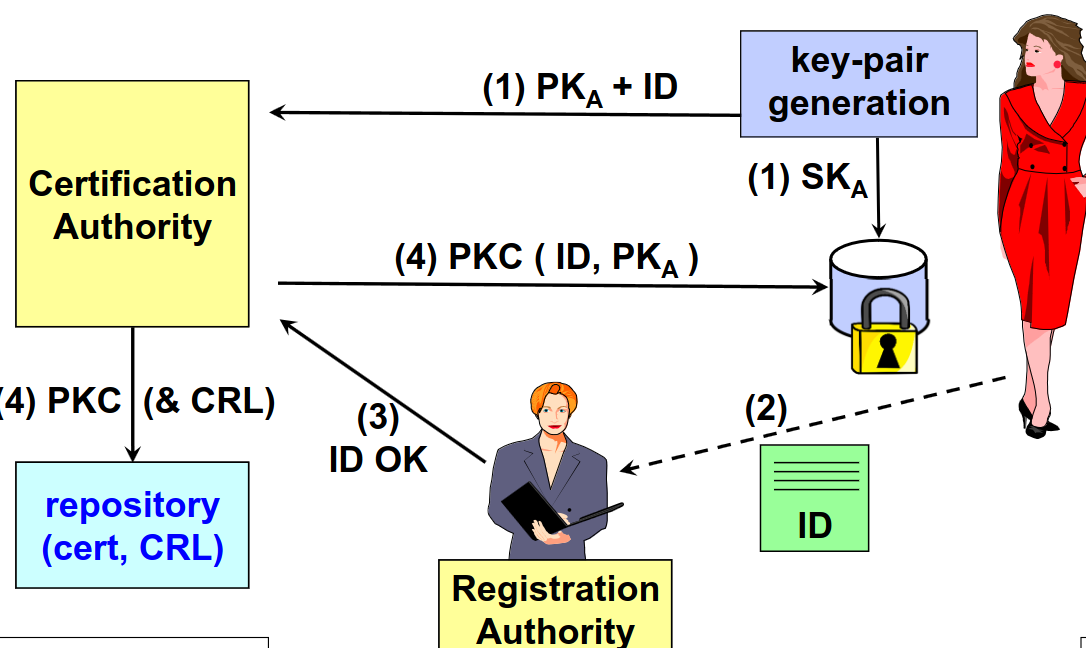
\includegraphics[width=0.95\textwidth]{./img/certificate-generation.png}
  \end{center}
  \caption{Certificate generation}\label{fig:certificate-generation}
\end{figure}
The Figure~\ref{fig:certificate-generation} is only one method of generation, maybe the RA generated the key-pair, obtains the PKC, and distribute them on a secure device (e.g. smart-cart), typycal for large companies.

\subsection{X.509}
It is a standard, which was part of the X.500 (for directory services), where to identify a leaf of a tree, we use the chain of nodes which is called \textbf{Distinguish Name} (DN).

The X.509 has some kind of problems related to how to identify an entity:
CP:
CPS:
CP is specification that may be followed by a CA, but thy might implement differnt CPS.

The standard was completed in 1996, used for internet application, and a document with all the extensions was released. 
Public extension: defined into the standard 
Private extension: the company or a community may put in the certificate additional infomation, the problem is that this is not standardized.
Certificate profile: set of extensions for a specific purposes

Pub:
- info about the key 
- attributes to identify issures and subject
- CRL distribution point 

Key and policy info:
- authority key identifier (AKI): specify a PK -> digest of the PK, issuer name and his serial number
- subjec key identifier: 
- key usage (KU): identifies the application domain for wich the public key can by used 
  - digitalSig
  - nonRepudiation 
  - dataEnchiperment
  - keyEnchiperment
  - keyAgreement
  - keyCertSign
  - CRL Sign
- private key usage period: with more time an attacker can break the private key
- certificate policies: list of policies which explains the purpose the certificate trought a: text, URI, ODI,
- policy mapping: common policies among certificates











\end{document}

%% vim: ts=2 sts=2 sw=2 et
